\documentclass[titlepage]{tufte-book}

\usepackage[runall=true]{pythontex}
\setpythontexworkingdir{<outputdir>}
\usepackage{environ}
\usepackage{morewrites}
\usepackage{amsthm}
\usepackage{amsmath}
\usepackage{amssymb}
\usepackage[pdftex]{graphicx}
\usepackage{epstopdf}
\usepackage{hyperref}
\usepackage{alltt}
\usepackage{listings}
\usepackage{array}
\usepackage{extarrows}
\usepackage{setspace}
\usepackage{tikz}
\usepackage{tikz-qtree}
\usetikzlibrary{calc}
\usetikzlibrary{positioning}
\usepackage{hyperref}
\usepackage{graphviz}
\usepackage{geometry}                % See geometry.pdf to learn the layout options. There are lots.
\usepackage{bashful}
\usepackage{microtype} % Improves character and word spacing
\usepackage{caption}

\usepackage{booktabs} % Better horizontal rules in tables

\setkeys{Gin}{width=\linewidth,totalheight=\textheight,keepaspectratio} % Improves figure scaling
\graphicspath{{figures/}}

\usepackage{fancyvrb} % Allows customization of verbatim environments
\fvset{fontsize=\normalsize} % The font size of all verbatim text can be changed here

\newcounter{problem}
\newcounter{total}
\newcommand{\step}[1]{{}
\vspace{4pt} \noindent {\bf \theproblem. }#1\addtocounter{problem}{1}}

\newcommand{\cut}[1]{}

\usepackage[tikz]{bclogo}
\usepackage{tikz}
\usetikzlibrary{calc}

\lstdefinestyle{BashInputStyle}{
  language=bash,
  basicstyle=\small\ttfamily,
  numberstyle=\tiny,
  showstringspaces=false,
  numbersep=3pt,
  otherkeywords={|, ;, ', ", *,>, <, *, &, `, $},
  alsoletter={:~_},
  columns=fullflexible,
  backgroundcolor=\color{yellow!20},
  linewidth=0.93\linewidth,
  xleftmargin=0.03\linewidth,
  keywordstyle=\color{blue},
  emph={ls, cat, head, tail, more, less, sort, uniq, kill java, grep, zip, unzip, tar, wc, cp, chmod,chown},
  emphstyle=\color{black}\bfseries,
    commentstyle=\color{gray}\slshape
    }

\newcommand{\chili}{\scalebox{.04}{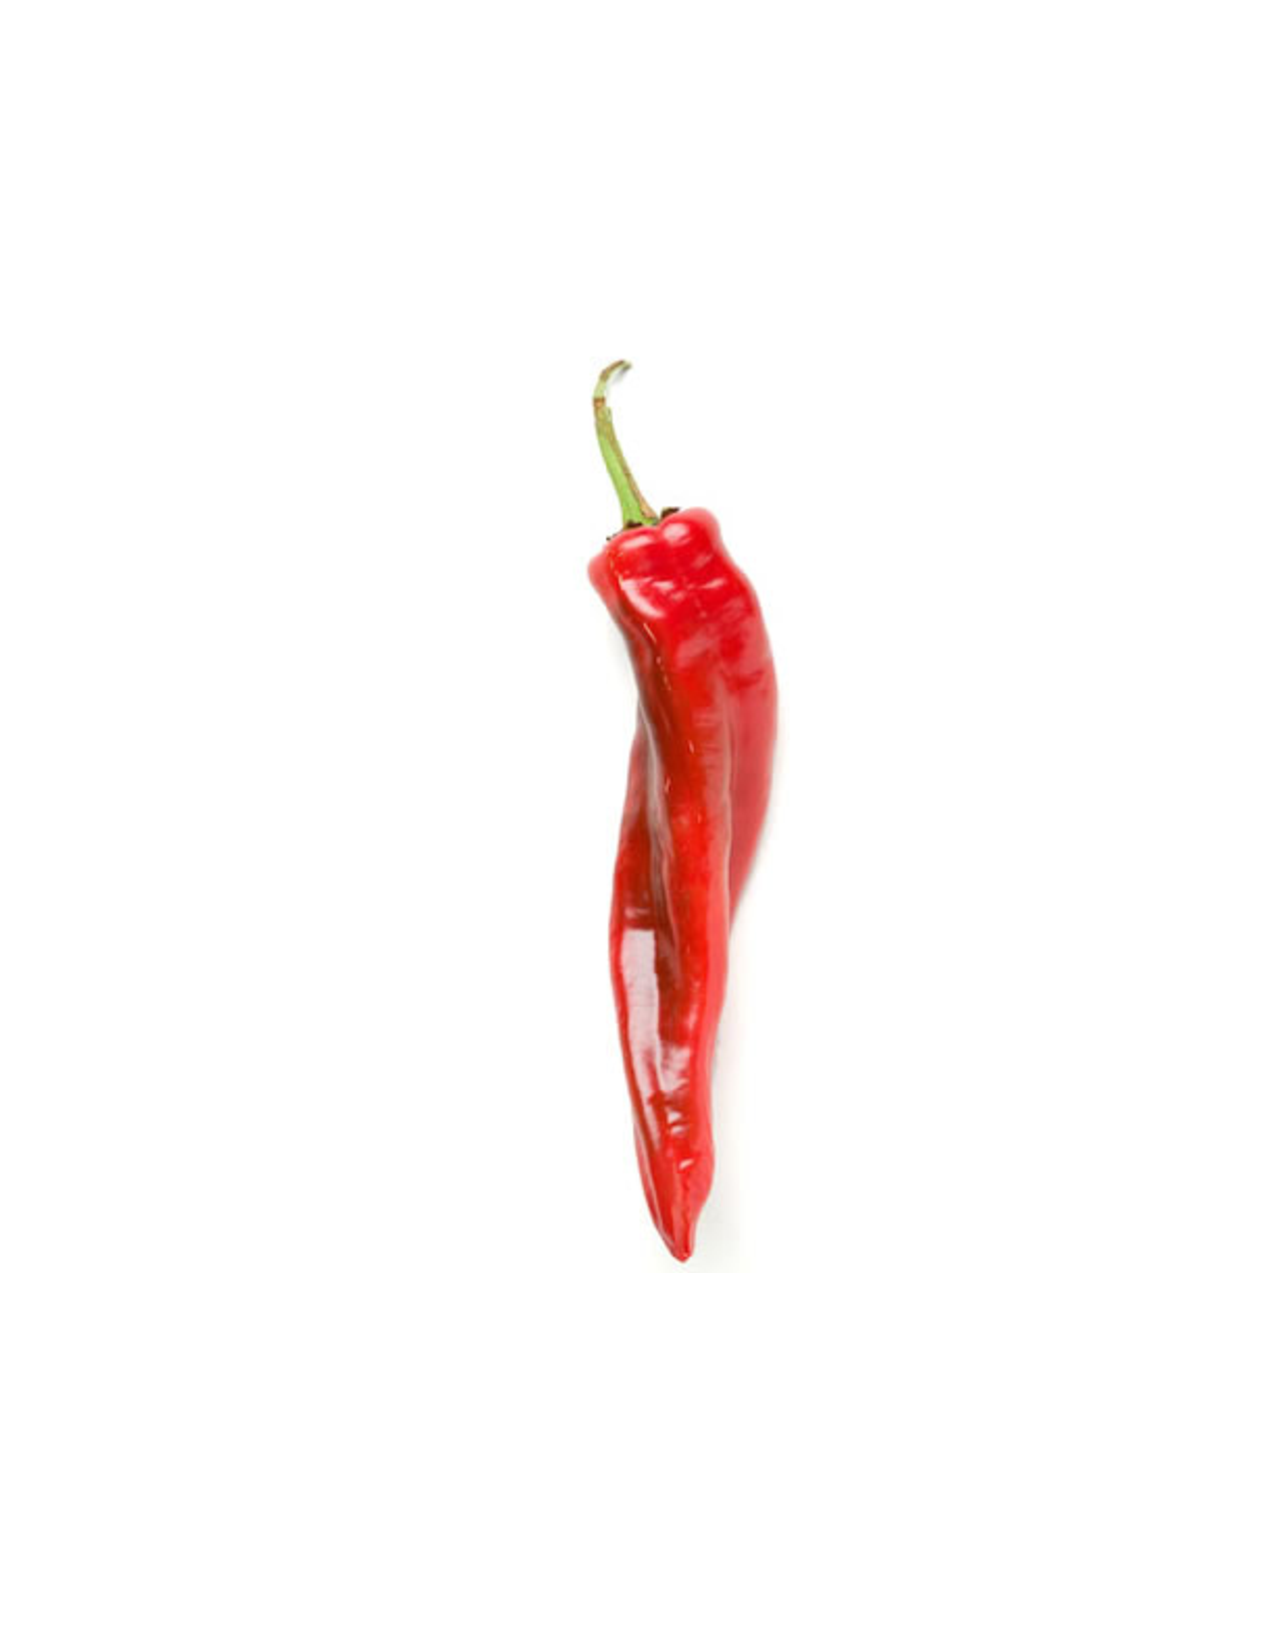
\includegraphics{figures/chili.pdf}}}
\newcommand{\chchili}{{\chili\chili}}
\newcommand{\chchchili}{{\chchili\chili}}

% The units package provides nice, non-stacked fractions and better spacing
% for units.
\usepackage{units}

% The fancyvrb package lets us customize the formatting of verbatim
% environments.  We use a slightly smaller font.
\usepackage{fancyvrb}
\fvset{fontsize=\normalsize}

% Small sections of multiple columns
\usepackage{multicol}

\hypersetup{
urlcolor=blue,
colorlinks=true
}
\usepackage[noline, procnumbered, linesnumberedhidden, boxed]{algorithm2e}

\newcommand{\openepigraph}[2]{ % This block sets up a command for printing an epigraph with 2 arguments - the quote and the author
\begin{fullwidth}
\sffamily\large
\begin{doublespace}
\noindent\allcaps{#1}\\ % The quote
\noindent\allcaps{#2} % The author
\end{doublespace}
\end{fullwidth}
}

\newcommand{\figref}[1]{Figure~\ref{#1}}
\renewcommand{\thefigure}{\arabic{figure}}

\newenvironment{callout}[1]{
\[
  \left[
      \begin{tabular}{@{\quad}m{.05\textwidth}@{\qquad}m{.75\textwidth}@{\quad}}
        \scalebox{1.5}{#1} & 
          \raggedright%
}
{
      \end{tabular}
    \right]
\]
}

\newcommand{\blankpage}{\newpage\hbox{}\thispagestyle{empty}\newpage} % Command to insert a blank page

\usepackage{makeidx} % Used to generate the index
\makeindex % Generate the index which is printed at the end of the document

\renewcommand{\maketitlepage}[0]{%
  \cleardoublepage%
  {%
  \sffamily%
  \begin{fullwidth}%
  ~
  \vspace{11.5pc}%
  \fontsize{36}{40}\selectfont\par\noindent\textcolor{darkgray}{\allcaps{\thanklesstitle}}%
  
\scalebox{.2}{\includegraphics{figures/msan-logo}}
  \vspace{11.5pc}%
  \fontsize{12}{18}\selectfont\par\indent\textcolor{darkgray}{\allcaps{\thanklessauthor}\\
\indent{\tt parrt@cs.usfca.edu}\\
\href{http://parrt.cs.usfca.edu}{http://parrt.cs.usfca.edu}}%
  \vspace{11.5pc}%
  \fontsize{14}{16}\selectfont\par\noindent\allcaps{\thanklesspublisher}%
  \end{fullwidth}%
  }
  \thispagestyle{empty}%
  \clearpage%
}

\titlecontents{part}% FIXME
    [0em] % distance from left margin
    {\vspace{1.5\baselineskip}\begin{fullwidth}\LARGE\rmfamily\itshape} % above (global formatting of entry)
    {\contentslabel{2em}} % before w/label (label = ``II'')
    {} % before w/o label
    {\rmfamily\upshape\qquad\thecontentspage} % filler + page (leaders and page num)
    [\end{fullwidth}] % after

  \titlecontents{chapter}%
    [0em] % distance from left margin
    {\vspace{1.5\baselineskip}\begin{fullwidth}\Large\rmfamily\itshape} % above (global formatting of entry)
    {\hspace*{0em}\contentslabel{2em}} % before w/label (label = ``2'')
    {\hspace*{4em}} % before w/o label
    {\rmfamily\upshape\qquad\thecontentspage} % filler + page (leaders and page num)
    [\end{fullwidth}] % after

\titlespacing*{\chapter}{0pt}{0pt}{30pt}
\titlespacing*{\section}{0pt}{3.5ex plus 1ex minus .2ex}{2.3ex plus .2ex}
\titlespacing*{\subsection}{0pt}{3.25ex plus 1ex minus .2ex}{1.5ex plus.2ex}

\begin{document}

\chapter{Image Processing}

\setcounter{problem}{1}

\noindent The goal of this project is to exercise your understanding of all of the major components in Python: {\bf assignments, expressions, if and loop statements, functions, lists, and libraries}. To make things interesting, we will perform some cool image processing tasks: {\bf flipping horizontally, blurring, removing salt-and-pepper image noise, finding edges within images, and image sharpening}.  For example, \figref{sharpbonkers} demonstrates image sharpening.

\begin{marginfigure}
\begin{center}
\scalebox{.45}{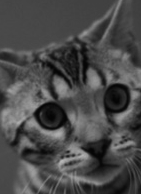
\includegraphics{figures/bonkers-bw-zoom.png}}
\scalebox{.45}{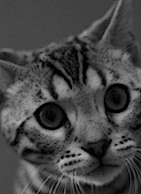
\includegraphics{figures/bonkers-sharp-zoom.png}}
\end{center}
\caption{Bonkers the cat sharpened using {\tt sharpen.py}.}
\label{sharpbonkers}
\end{marginfigure}

\section{Git from the command line}

Let's prepare our programming environment so that submitting this project is easy.  This process is abbreviated here, but you can see it fleshed out in more detail in the section "Getting Started On The Images Project" of the \href{https://github.com/parrt/msan501/blob/master/notes/git.md}{\textcolor{blue}git lecture}.

I will post to slack or via the students email list a URL for each project that represents an invitation to create a repository associated with a specific project for this class. Each student will have their own private repository per project. Once you have created the repository, you can proceed with this section to clone that empty repository onto your laptop disk.

Launch Terminal.app or whatever your bash shell is called on your system. Now, using a browser, go to the URL associated with your images project at github, which should be something like (YOURID is your github user/id not your laptop username): 

{\tt https://github.com/YOURID/images-YOURID}

\noindent and copy the {\tt HTTPS not SSH} URL from here:

\scalebox{.5}{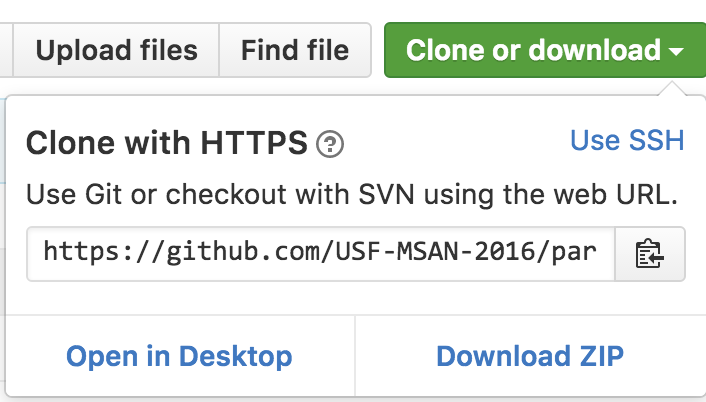
\includegraphics{figures/github-url.png}}

\noindent (That graphic is a bit out of date and the URL will look different in that little text field.) Then, use the {\tt git clone }{\em URL} command as you see below, replacing {\tt images-parrt} with {\tt images}-{\em yourid}. You will have to type in your github user ID and password.

\begin{lstlisting}[style=BashInputStyle]
$ cd ~/msan501 #  assuming this is where you want the root of all of 501 projects
$ git clone https://github.com/USF-MSAN-2016/images-parrt.git
Cloning into 'images-parrt'...
Username for 'https://github.com': parrt
Password for 'https://parrt@github.com': 
remote: Counting objects: 19, done.
remote: Compressing objects: 100% (6/6), done.
remote: Total 19 (delta 0), reused 0 (delta 0), pack-reused 13
Unpacking objects: 100% (19/19), done.
Checking connectivity... done.
$ cd images-parrt # after this command you are now in your repository
\end{lstlisting}

\noindent There is nothing in the repo yet, but we'll get to it!

\section{Getting started}

To get started, review how to access the \href{http://stackoverflow.com/questions/4117530/sys-argv1-meaning-in-script}{\textcolor{blue}{command-line arguments}} that every program running on a computer can accept. Here is a small program, {\tt view.py}, that accepts a filename as a command-line argument. The goal is really just to ensure that the PIL library is available for use, which you should be because you're using the Anaconda icon installation.

\begin{pyverbatim}
import sys
from PIL import Image
if len(sys.argv) != 2:
	print "$ python view.py imagefilename"
	sys.exit(1)
filename = sys.argv[1] # get the argument passed to us by operating system
img = Image.open(filename) # load file specified on the command line
img = img.convert("L") # grayscale
img.show()
\end{pyverbatim}

\noindent (I provide this file and another in the \href{https://github.com/parrt/msan501-starterkit/tree/master/images}{\textcolor{blue}{starter kit}}.)

To run this program, launch a terminal on Mac or Linux. Then, move to the directory that contains {\tt view.py} that you saved/typed-in using terminal command {\tt cd} (change directory).  For example, if you are using directory {\tt msan501/images-yourid} under your home directory for this project, then type this:

\begin{lstlisting}[style=BashInputStyle]
cd ~/msan501/images-yourid; # ~ character is shorthand for /Users/yourid
\end{lstlisting}

You can get a \href{https://github.com/parrt/msan501/tree/master/projects/figures}{\textcolor{blue}{bunch of sample images}} that I use for these notes from github, but of course you can play around with whatever images you want.\sidenote{Remember, however, that all images used in this class and those stored on University equipment must be ``safe for work.'' Keep it G-rated please, with no offensive images popping up on your laptops or machines during lab etc.}

Now, we can execute our {\tt view.py} script and pass it an argument of {\tt obama.png}:

\begin{lstlisting}[style=BashInputStyle]
$ python view.py obama.png
\end{lstlisting}

If you are using PyCharm, you need to right-click in the code editor and say ``run view.py,'' which will ``fail'' with this message in the Run tab:

\begin{alltt}
/usr/local/bin/python /Users/parrt/github/msan501/projects/code/images/view.py
$ python view.py imagefilename
\end{alltt}

\noindent Now, use the ``{\tt\small Edit configuration}'' dialog under the {\tt Run} menu.  All file names that we specify in the script parameters area, or from the command line, are relative to the {\em current working directory}. That is why we used {\tt cd} to change our working directory in the example above. For convenience, keep all of images and scripts in the same directory. For our purposes, let's assume that the directory is always {\tt\small /Users/YOURID/msan501/images-YOURID} (Mac) or {\tt\small /home/YOURID/msan501/images-YOURID} (Linux).   Here is the dialogbox for editing the run configuration, where my {\tt view.py} file is in my {\tt ~/github/msan501-starterkit/images} directory:

\scalebox{1}{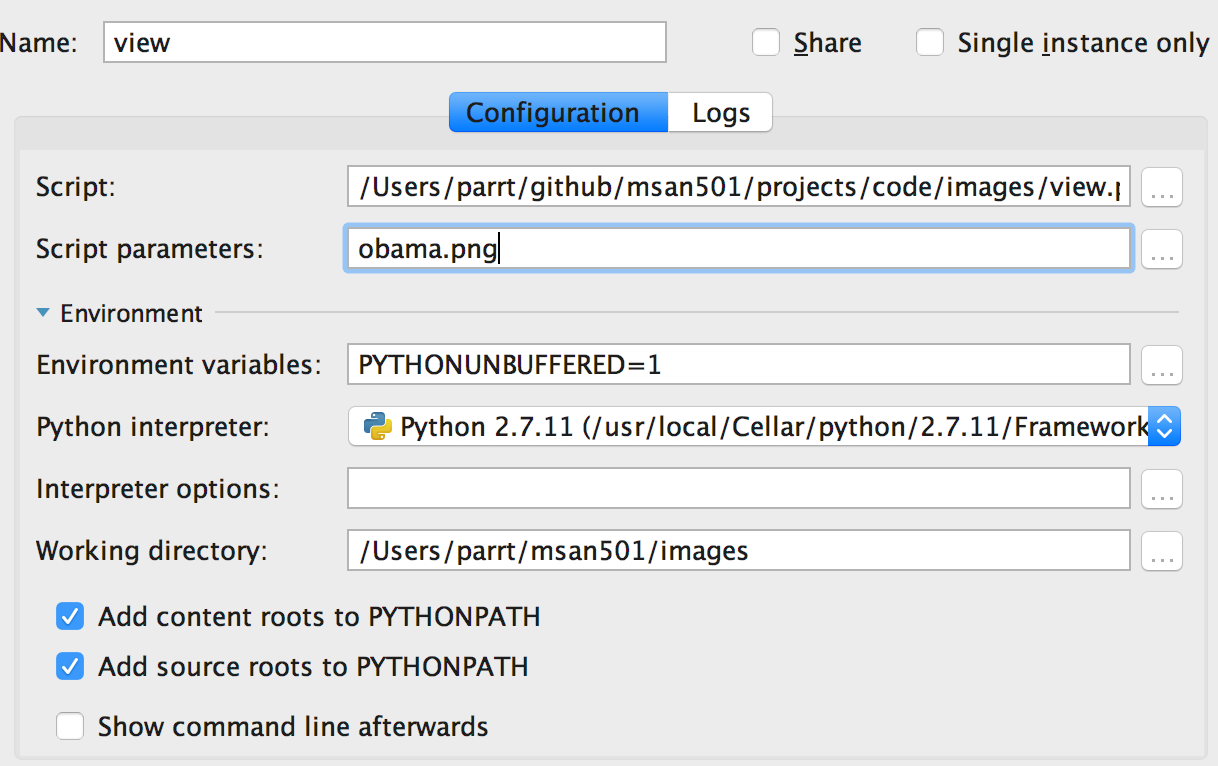
\includegraphics{figures/edit-config.png}}

The ``Script parameters'' text field is where you provide the ``command-line arguments,'' despite the fact we are not actually using a command-line. That is why PyCharm calls it script parameters instead of command-line parameters. Also note that it is running with anaconda's Python, which has the imaging library preinstalled!

Now, if you click the "run" button, you will see Obama's image appear on your screen or the "eyes" if you use {\tt eye.png}.

\section{Task 1. Flipping an image horizontally}

As a first task,  create a script called {\tt flip.py} that shows the image provided as a program (command-line) argument in its original form and then flipped horizontally.  For example, \figref{flipped} shows the result of running script {\tt flip.py} on image {\tt eye.png}.

\begin{marginfigure}
\begin{center}
\scalebox{.49}{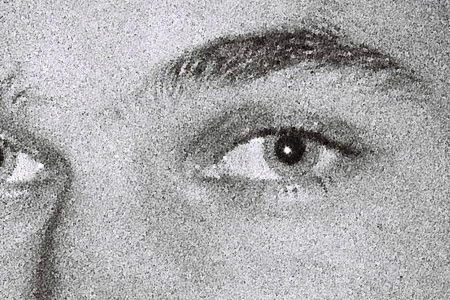
\includegraphics{figures/eye.png}} \scalebox{.49}{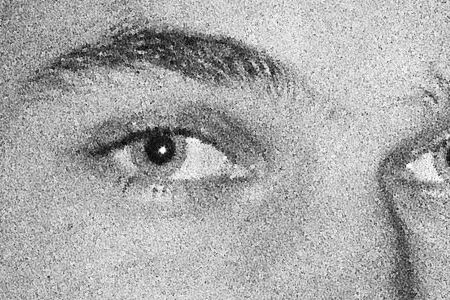
\includegraphics{figures/eye-flip.png}}
\end{center}
\caption{Flipping an image horizontally; the original is on the left.}
\label{flipped}
\end{marginfigure}

\subsection{Boilerplate code}

Here's the boilerplate or ``skeleton'' code from:

\href{https://github.com/parrt/msan501-starterkit/tree/master/images/flip.py}{\tt\small https://github.com/parrt/msan501-starterkit/tree/master/images/flip.py}

\noindent that we already know how to do but with a hole where you need to define a function called {\tt flip} and a hole where you need to call that function to perform the flipping:

\begin{pyverbatim}
import sys
from PIL import Image

# define your flip function here
...
if len(sys.argv)<=1:
	print "missing image filename"
	sys.exit(1)
filename = sys.argv[1]
img = Image.open(filename)
img = img.convert("L")
img.show()

# call your flip function here
...
img.show()
\end{pyverbatim}

An explanation of how to fill in those holes appears shortly.

\subsection{Adding files to your repo}

After creating the {\tt flip.py} file and copying over an image or two, your PyCharm project file list area should look like the list in \figref{fliplist}.  So that git will manage our project, we need to announce that git should track {\tt flip.py}:


\begin{marginfigure}
\begin{center}
\scalebox{.8}{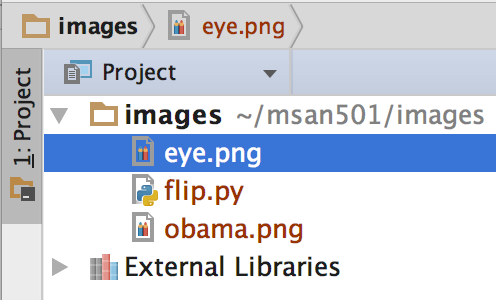
\includegraphics{figures/flip-proj-browser.png}}
\end{center}
\caption{Project file list after creating the flip.py file}
\label{fliplist}
\end{marginfigure}

\begin{lstlisting}[style=BashInputStyle]
$ cd ~/msan501/images-yourid
... copy image files, create flip.py ...
$ git add flip.py
\end{lstlisting}

Note that, if you are using PyCharm, when you open the dir in PyCharm, it will notice that the dir is a git repo. You can use PyCharm to manage the git repository later when you get more experience, but let's do things explicitly now from the command line.

Even though we haven't done any work on {\tt flip.py} yet, let's commit the file to the repository and then push the repository back to github:

\begin{lstlisting}[style=BashInputStyle]
$ git commit -a -m 'add eye flip boilerplate code'
[master adcf1df] add eye flip boilerplate code
...
$ git push origin master
...
\end{lstlisting}

Now, go check out that github has the files. The web page for your repository should look something like the following, but without the images:

\scalebox{.9}{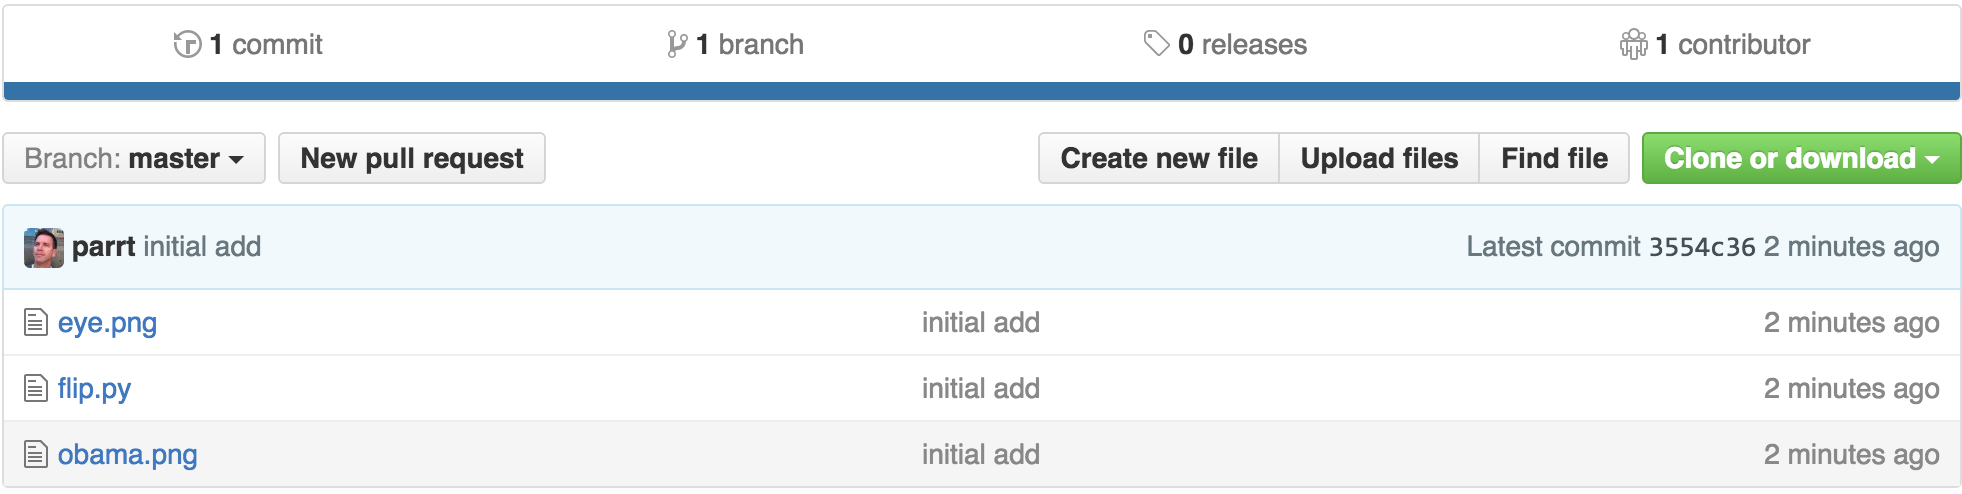
\includegraphics{figures/github-initial-add.png}}

\subsection{Three new Pillow pieces}

To write your {\tt flip} function, you will need three basic pieces:

\begin{itemize}
\item {\tt img.size} returns a tuple containing the width and height of image {\tt img} so you can write code like this:
\begin{pyverbatim}
width, height = img.size
\end{pyverbatim}
You'll need the width and height to iterate over the pixels of the image.

\item {\tt img.copy()} duplicates image {\tt img}.  For our {\tt flip} function, it would be hard to modify the image in place because we would be overwriting pixels we would need to flip later. It's easier to create a copy of the image in flipped position. You can write code like this:\\
{\tt imgdup = img.copy()}

\item {\tt img.load()} is yet another weird name from PIL that actually returns an object that looks like a two-dimensional matrix, which is really just a lists of lists such as {\tt m = [[1,2], [3, 4]]}. When printed, the output looks like a matrix:

\begin{pyverbatim}
m = [[1, 2],
     [3, 4]]
\end{pyverbatim}
To get element {\tt 3}, we would use list index expression {\tt m[1][0]} because we want the list at index 1, {\tt m[1]}, and then element 0 within that list. The two-dimensional object returned by {\tt load()} uses similar notation. If we ask for the ``matrix'' with:
\begin{pyverbatim}
m = img.load()
\end{pyverbatim}
then we  use notation {\tt m[x,y]} to get the pixel at position ({\tt x}, {\tt y}).
\end{itemize}

You will use these functions for the remaining tasks so keep them in mind.

\subsection{Iterating over the image matrix}

{\bf Define function} {\tt flip} using the familiar function definition syntax and have it take a parameter called {\tt img}, which will be the image we want to flip. The goal is to create a copy of this image, flip it, and return a copy so that we do not alter the incoming original image. To create {\tt flip}, write code that implements the following steps.

\begin{enumerate}
\item Use {\tt size} to define local variables {\tt width} and {\tt height}
\item Use {\tt copy()} to make a copy of the incoming image {\tt img} and save it in a local variable
\item Use {\tt load()} to get the two-dimensional pixel matrix out of the incoming image and the copy of the image. Store these results in two new local variables.
\item To walk over the two-dimensional image, we've learned we need every combination of {\tt x} and {\tt y}. That means we need a nested {\tt for} loop. Create a nested for loop that iterates over all {\tt x} and all {\tt y} values within the {\tt width} and {\tt height} of the image.
\item Within the inner loop, set pixels in the image copy to the appropriate pixel copied from the original image
\item At the end of the function, return the flipped image
\end{enumerate}

The only remaining issue is determining which pixel from the original image to copy into the ({\tt x}, {\tt y}) position in the image copy. The {\tt y} index will be the same since we are flipping horizontally. The {\tt x} index in the flipped image is index {\tt width-x-1} from the original image. Trying out a few sample indexes shows that this works well. For example, a flipped image with {\tt width=10} has its pixel at {\tt x=0} pulled from index {\tt x=10-0-1=9} in the original image. That's great, because it takes the image from all in the right in the original and copies it to the far left of the copy. Checking the opposite extreme, {\tt x=9} in the flipped image should be {\tt x=10-9-1=0} from the original image.

\subsection{Running your flip script}

{\bf To run the script from the command line}, make sure you are in the {\tt msan501/images-userid} directory containing your scripts and images then do:

\begin{lstlisting}[style=BashInputStyle]
$ cd msan501/images-userid
$ python flip.py eye.png
\end{lstlisting}

{\bf From PyCharm}, I right-click and then select ``Run.'' It will do nothing but print ``{\tt missing image filename}'' because we have not given it a parameter yet, but we need to do this so that PyCharm creates a run configuration. Now, use the edit configuration dialog to specify {\tt eye.png} as a parameter or any other image. ({\em Remember that the filename must refer to a file in the current working directory or must be fully qualified.}) Click ``Run'' now and it should bring out the two images. The dialog box will look something like this:

\scalebox{.9}{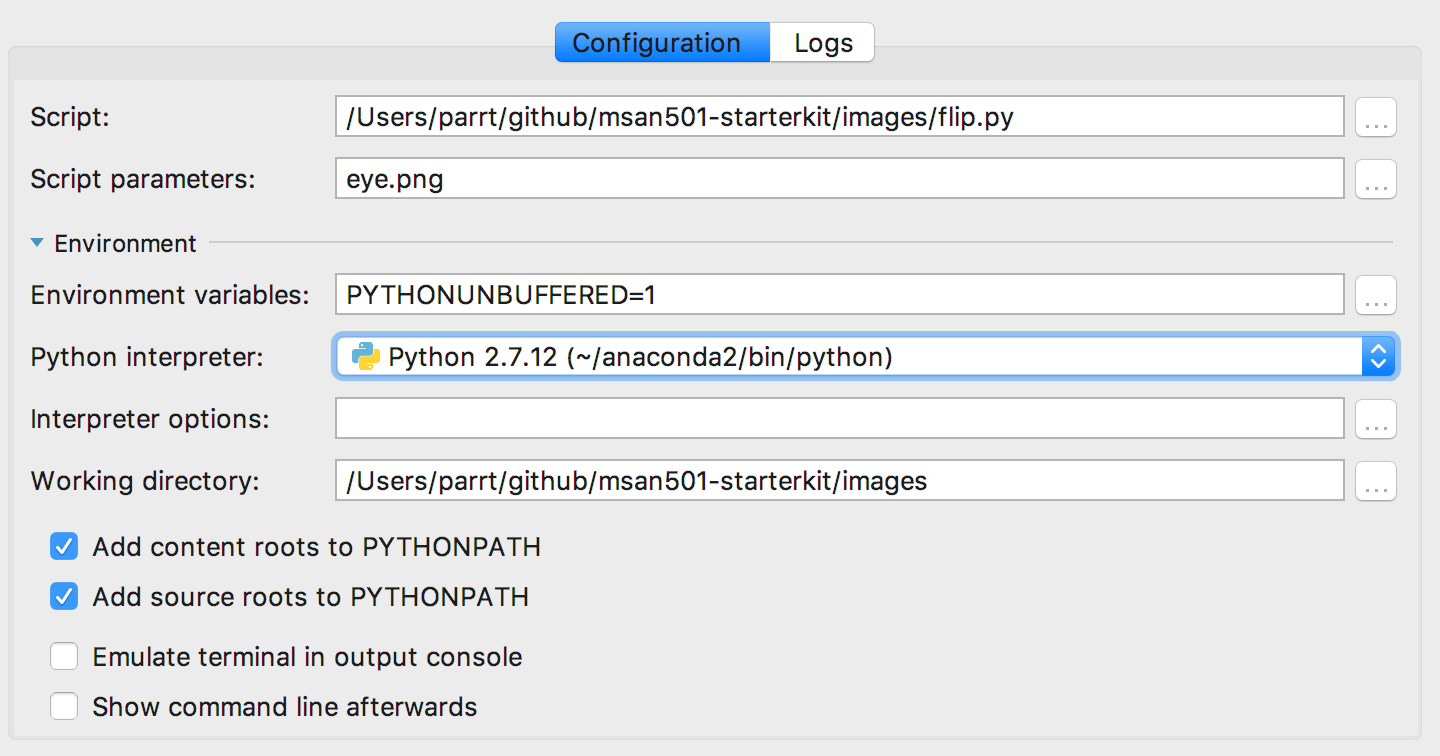
\includegraphics{figures/flip-config.png}}

Again, please make sure that you are using the Anaconda Python so that it has the appropriate image processing libraries.

\subsection{What to do when the program doesn't work}

If you have problems, follow these steps:

\begin{enumerate}
\item Don't Panic! Relax and realize that you will solve this problem, even if it takes a little bit of messing around. Banging your head against the computer is part of your job. Remember that the computer is doing precisely what you tell it to do. There is no mystery.
\item  Determine precisely what is going on. Did you get an error message from Python?  Is it a syntax error? If so, review the syntax of all your statements and expressions. PyCharm is your friend here and should highlight erroneous things with a red squiggly underline. If you got an error message that has what we call a stack trace, a number of things could be wrong. For example, if I misspell {\tt show()} as {\tt shower()}, I get the following message:
\begin{alltt}\small
Traceback (most recent call last):
  File "/Users/parrt/msan501/images-parrt/flip.py", line 26, in <module>
    img.shower()
  File "/usr/local/lib/python2.7/site-packages/PIL/Image.py", line 605, in __getattr__
    raise AttributeError(name)
AttributeError: shower
\end{alltt}
In PyCharm, the ``{\tt /Users/parrt/msan501/images-parrt/flip.py}'' part of the trace will be a blue link that you can click on. It will take you to the exact location in your script where there is a problem. Look for anything that refers to that file.
\item If it does not look like it some simple misspelling, you might get lucky and find something in Google if you cut-and-paste that error message.
\item If your script shows the original image but not the flipped image, then you likely have a problem with your {\tt flip} function.
\item If your program is at least running and doing something, then insert print statements to figure out what the variables are and how far into the program you get before a craps out. That often tells you what the problem is.
\item Try using the debugger to step through your program in PyCharm. Set a breakpoint on for example the line {\tt filename = sys.argv[1]} by clicking in the gutter to the left of that line.  A red dot should appear, indicating there is a breakpoint there. Then click the little bug icon instead of the green triangle (which is run button). That will start execution and then stop at that line. You can look at all of the variables at that point. Then you can step forward line by line. Read how to use the debugger online.
\item  Definitely try to solve the problem yourself, but don't waste too much time. I can typically help you out quickly so you can move forward.
\end{enumerate}

\begin{callout}{\bcplume}
{\bf Deliverables}. Make sure that {\tt images-}{\em userid}{\tt /flip.py} is correctly committed to your repository and pushed to github. 
\end{callout}

\section{Task 2. Blurring}

In this task, we want to blur an image by removing detail as shown in \figref{blur}. We will do this by creating a new image whose pixels are the average of the surrounding pixels for which we will use a 3x3 region as shown in \figref{region}. The pixel in the center of the region is the region to compute as we slide the region around an image. In other words, {\tt pixel[x,y]} is the sum of {\tt pixel[x,y]} and all surrounding pixels divided by 9, the total number of pixels.

\begin{marginfigure}
\begin{center}
\scalebox{.87}{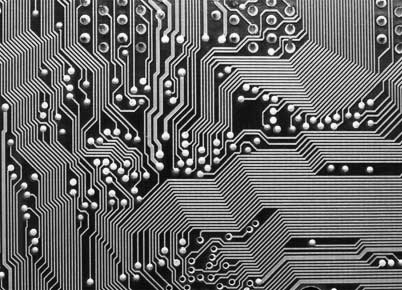
\includegraphics{figures/pcb.png}}\\
\scalebox{.87}{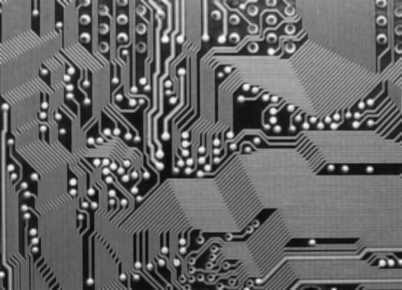
\includegraphics{figures/pcb-blur.png}}
\end{center}
\captionof{figure}{Blurring of a circuit board; the original is on top.}
\label{blur}
\end{marginfigure}

To implement this, start with the boilerplate from the previous section, which you should put into script {\tt blur.py}. The only difference is that you must call soon-to-be-created function {\tt blur} not {\tt flip} as you had before. Now, let's start at the coarsest-level of functionality and realize that we have to walk over every pixel in the image. (This is called {\em top-down design}.) 

\subsection{Blurring function}

{\bf Define function} {\tt blur} to take an {\tt img} parameter, just like the {\tt flip} function in the previous task.  In a manner very similar to {\tt flip}, write code in {\tt blur} to accomplish these steps:

\begin{enumerate}

\item Define local variables {\tt width} and {\tt height}.
\item Make a copy of the incoming image {\tt img} and save it in a local variable.
\item Get the two-dimensional pixel matrix out of the image copy. Store it in a new local variable called {\tt pixels}.
\item Create a nested for loop that iterates over all {\tt x} and all {\tt y} values within the {\tt width} and {\tt height} of the image.
\item Within the inner loop:
\begin{enumerate}
\item Call to-be-created function {\tt region3x3} with arguments {\tt img}, {\tt x}, and {\tt y} in store into local variable {\tt r}.
\item Set {\tt pixels[x,y]} in the image copy to the result of calling to-be-created function {\tt avg} with an argument of {\tt r}.
\end{enumerate}
\item At the end of the function, return the blurred image.
\end{enumerate} 

Following the top-down design strategy, let's {\bf define function} {\tt avg} since it's the easiest. Define {\tt avg} to take an argument called {\tt data} or another of your choice. This will be the list of 9 pixels returned by function {\tt region3x3}. The average of a set of numbers is their total divided by how many numbers there are. Python provides two useful functions here: {\tt sum(data)} and {\tt len(data)}.  (Naturally, {\tt sum} simply walks the list and accumulates values using a pattern we are familiar with.)

\subsection{Image regions}

Now we need to {\bf define function} {\tt region3x3}.  Have it take three parameters as described above. This function creates and {\bf return a list of nine pixels}. The list includes the center pixel at {\tt x}, {\tt y} and the 8 adjacent pixels at N, S, E, W, ... as shown in \figref{region}. Create a series of assignments that look like this:

\begin{marginfigure}
\begin{center}
\scalebox{1}{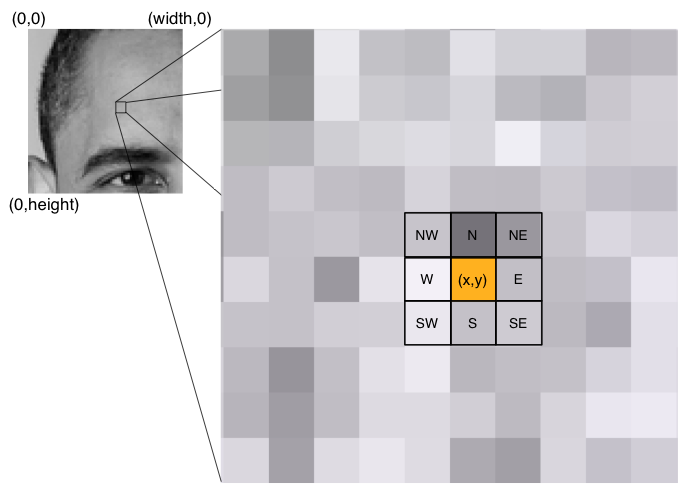
\includegraphics{figures/region.png}}
\end{center}
\captionof{figure}{Hyper-zoom of Obama's forehead showing 3x3 region.}
\label{region}
\end{marginfigure}

\begin{pyverbatim}
me = getpixel(img, x, y)
N = getpixel(img, x, y - 1)
...
\end{pyverbatim}

\noindent where function {\tt getpixel(img, x, y)} gets the pixel at {\tt x}, {\tt y} in image {\tt img}.  We can't use the more readable expression {\tt pixels[x,y]} in this case, as we'll see in a second. Collect all those pixel values into a list using {\tt [a,b,c,...]} list literal notation and return it. Make sure that this list is a list of integers and exactly 9 elements long and that you keep in mind the order in which you add these pixels to the list. Any function that we create to operate on a region naturally needs to know the order so we can properly extract pixels from the list. For example, my implementation always puts the pixel at {\tt x} and {\tt y} first, then North, etc...

\subsection{Safely examining region pixels}

We need to {\tt define a function} {\tt getpixel} instead of directly accessing pixels because some of the pixels in our 3x3 region will be outside of the image as we shift the region around. For example, when we start out at {\tt x=0}, {\tt y=0}, 5 of the pixels will be out of range, as shown in \figref{outofrange}.  Accessing {\tt pixels[-1,-1]} will trigger:

\begin{marginfigure}
\begin{center}
\scalebox{.85}{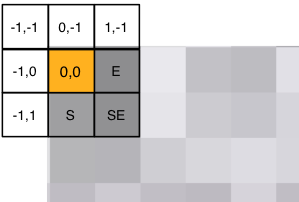
\includegraphics{figures/region-edge.png}}
\end{center}
\captionof{figure}{Our 3x3 region has pixels outside of the image boundaries as we slide it around the image along the edges.}
\label{outofrange}
\end{marginfigure}

{\tt IndexError: image index out of range}

\noindent and stop the program. To avoid this error and provide a suitable definition for the ill-defined pixels on the edges, we will use a function that ensures all indices are within range.

{\bf Define function} {\tt getpixel} with the appropriate parameters. Its functionality is as follows:
\begin{enumerate}
\item Get the width and height into local variables.
\item If the {\tt x} value is less than 0, set it to 0.
\item If the {\tt x} value is greater than or equal to the width, set it to the width minus 1 (the last  valid pixel on the far right).
\item If the {\tt y} value is less than 0, set it to 0.
\item If the {\tt y} value is greater than or equal to the height, set it to the  height minus 1 (the last felt pixel on the bottom).
\item Return the pixel at {\tt x}, {\tt y}. You will need to use the {\tt img.load()} function again to get the 2D {\tt pixels} matrix as you did in function {\tt blur}. Make sure you returning pixel and not the coordinates of the pixel from {\tt getpixel}.
\end{enumerate}

\subsection{Testing your blur code}

That is a lot of code to enter and so more than likely it won't work the first time.\sidenote{It never does, dang it!} That means we should test the pieces. It's generally a good idea to do top-down design but {\em bottom-up testing}. In other words, let's test the simple low-level functions first and make sure that works before testing the functions that call those functions and so on until we reach the outermost script. 

With that in mind, lets test {\tt avg} by passing it a fixed list of numbers to see if we get the right number. Add this to your script before it does any of the file loading stuff:

\begin{pyverbatim}
print avg([1,2,3,4,5])
\end{pyverbatim}

\noindent Then run {\tt blur.py} with any old image; the {\tt apple.png} file is a good one because it's small (it's in the {\tt projects/figures} dir of the {\tt msan501} repo):

\begin{lstlisting}[style=BashInputStyle]
$ python blur.py apple.png
3
$ 
\end{lstlisting}

\noindent If it does not print $(1+2+3+4+5)/5 = 3$, then you know you have a problem in {\tt avg}.

Now test {\tt getpixel}. You will have to insert some code after loading and converting the image to grayscale because {\tt getpixel} takes an image parameter:

\begin{pyverbatim}
img = Image.open(filename)
img = img.convert("L")
print getpixel(img, 0, 0)
print getpixel(img, 0, 1)
print getpixel(img, 10, 20)
\end{pyverbatim}

\noindent  That should print: 96, 96, and 255. The upper left corner is gray and pixel 10, 20 is somewhere in the middle of the white Apple logo. If you don't get those numbers, then you have a problem with {\tt getpixel}. Worse, if you don't get simple numbers, then you really have a problem with {\tt getpixel}.

Before getting to {\tt blur}, we should also {\bf test} {\tt region3x3} to ensure it gets the proper region surrounding a pixel. Replace those {\tt getpixel} calls in the {\tt print} {\tt getpixel} statements with calls to {\tt region3x3}. Use the {\tt x}, {\tt y} of the upper left-hand corner and somewhere near the upper left of the white section of the logo such as:

\begin{pyverbatim}
print region3x3(img, 0, 0)
print region3x3(img, 7, 12)
\end{pyverbatim}

\noindent That checks whether we get an out of range error at the margins and that we get the correct region from somewhere in the middle. Running the script should give you the following numbers:

\begin{lstlisting}[style=BashInputStyle]
$ python blur.py apple.png
[96, 96, 96, 96, 96, 96, 96, 96, 96]
[255, 176, 255, 255, 215, 96, 245, 255, 255]
$ 
\end{lstlisting}

\noindent That assumes order: current pixel, N, S, E, W, NW, NE, SE, SW.

When you have verified that all of these functions work, it's time to check function {\tt blur} itself. Try the printed circuit board image:

\begin{lstlisting}[style=BashInputStyle]
$ python blur.py pcb.png 
\end{lstlisting}

\noindent That should pop up the original circuit board and the blurred version. It might take 10 seconds or more to compute and display the blurred image, depending on how fast your computer is.

\begin{callout}{\bctakecare}
Make sure to remove all of your debugging code before submitting your scripts. Submitting a project that prints out a bunch of random debugging output is considered sloppy, like submitting an English paper with a bunch of handwritten edits.
\end{callout}

\begin{callout}{\bcplume}
{\bf Deliverables}. Make sure that {\tt images-}{\em userid}{\tt /blur.py} is correctly committed to your repository and pushed to github.
\end{callout}

\section{Task 3. Removing noise}

\begin{marginfigure}
\begin{center}
(a) \scalebox{.5}{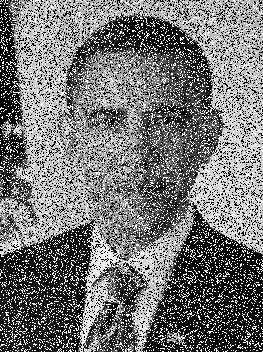
\includegraphics{figures/guesswho.png}}\\
(b) \scalebox{.5}{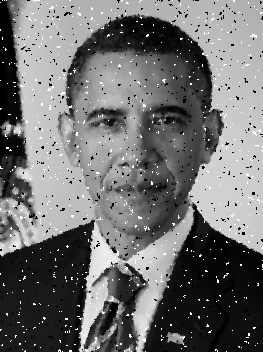
\includegraphics{figures/guesswho-denoise.png}}\\
(c) \scalebox{.5}{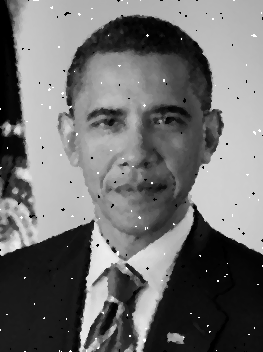
\includegraphics{figures/guesswho-denoise-denoise.png}}\\
(d) \scalebox{.5}{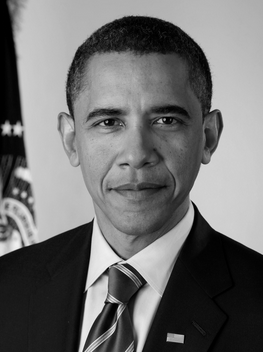
\includegraphics{figures/obama.png}}
\end{center}
\captionof{figure}{Denoising an image of President Obama with lots of salt-and-pepper noise. (a) the noisy image, (b) denoised as computed by {\tt denoise.py}, (c) denoised 2x, (d) original.}
\label{obama}
\end{marginfigure}

For our next task, we are going to de-noise (remove noise) from an image as shown in \figref{obama}. It does a shockingly good job considering the simplicity of our approach. To blur, we used the average of all pixels in the region. To denoise, we will use the \href{http://en.wikipedia.org/wiki/Median}{\textcolor{blue}{median}}, which is just the middle value in a list of ordered numbers.

Believe it or not, we can implement de-noise by copying {\tt blur.py} into a new script called {\tt denoise.py} and then changing a few lines.  We also have to remove the no-longer-used {\tt avg} function and replace it with a {\tt median} function.  Of course, instead of calling {\tt blur}, we'll call function {\tt denoise} with the usual {\tt img} argument. The only difference between {\tt denoise} and {\tt blur} is that you will set the pixel to the {\tt median} not {\tt avg}.  Hint: you need to tweak one statement in the inner loop that moves over all pixel values.

{\bf Now define function} {\tt median} that, like {\tt avg}, takes a list of 9 numbers called {\tt data}. Sort the list using Python's {\tt sorted} function, which takes a list and returns a sorted version of that list. Then compute the index of the middle list element, which is just the length of the list divided by two. If the length is even, dividing by 2 (not 2.0) will round it down to the nearest index. Once you have this index, return the element at that index.


Let's give it a test:

\begin{lstlisting}[style=BashInputStyle]
$ python denoise.py guesswho.png
\end{lstlisting}

\noindent That should pop up the noisy Obama and the cleaned up version. You can save the cleaned up version and run {\tt denoise.py} on that one to really improve it.\sidenote[][.5in]{Hint: {\bf To save an image with PIL}, use {\tt img.save("filename.png")}.} Running {\tt denoise.py} twice, gives the cleaned up image (c) from \figref{obama}.  

\begin{callout}{\bcplume}
{\bf Deliverables}. Make sure that {\tt images-}{\em userid}{\tt /denoise.py} is correctly committed to your repository and pushed to github. 
\end{callout}

\vspace{10mm}
\section{Task 4. Re-factoring to improve code quality}

As I mentioned in the last task, {\tt blur.py} and {\tt denoise.py} are virtually identical, meaning that we have a lot of code in common. \figref{vizdiff} demonstrates this visually. One of the most important principles of computer science is to reduce code duplication. We always want exactly one place to change a particular bit of functionality.   In this case, we have the following common code:

\begin{marginfigure}
\begin{center}
\scalebox{.95}{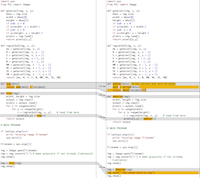
\includegraphics{figures/blur-denoise-diff.png}}
\end{center}
\caption{Visual difference between scripts {\tt blur.py} and {\tt denoise.py}. The files are identical except for orange marks.}
\label{vizdiff}
\end{marginfigure}

\begin{enumerate}
\item Functions {\tt getpixel} and {\tt region3x3}.
\item The ``main'' part of the script that loads the original image.
\item Functions {\tt blur} and {\tt denoise} are identical except for the function called to compute a new pixel in the image copy from a 3x3 region in the original ({\tt avg} or {\tt median}).
\end{enumerate}

The goal of this task is to make new versions, {\tt blur2.py} and {\tt denoise2.py}, that share as much code as possible.  The functionality will be the same, but they will be much smaller and we will get warm feeling that our code is well structured. To share code, we need to (a) put all common code in a file that these new scripts can import and (b) create a generic function called {\tt filter} that will work for both blurring and de-noising in an image. Once we get the common code into a single file, which we will call {\tt filter.py}, we can import it into {\tt blur2.py} and {\tt denoise2.py} like this:\sidenote{Do not confuse script names with function names; {\tt filter.py} can contain anything we want and it so happens that we will also put a function in there with the same name, {\tt filter}.}
 
\begin{pyverbatim}
from filter import *
\end{pyverbatim}

\noindent That statement asks Python to look in the current directory (among other places we don't care about for now) for file called {\tt filter.py} and import all of the functions. You can think of it as a formalized cut-and-paste.

Let's start by creating new ``library'' file {\tt filter.py} and placing our usual imports at the top:

\begin{pyverbatim}
import sys
from PIL import Image
\end{pyverbatim}

\noindent Now, copy functions {\tt getpixel} and {\tt region3x3} into it.

We can also create a function called {\tt open} to hide all of the messiness that checks for command-line arguments and opens the indicated image:

\begin{pyverbatim}
def open(argv):
	if len(argv)<=1:
		print "missing image filename"
		sys.exit(1)
	img = Image.open(argv[1])
	img = img.convert("L")  # make greyscale if not already (luminance)
	return img
\end{pyverbatim}

The only tricky bit\sidenote{Pun intended} is to create a single generic {\tt filter} function that can reproduce the functionality we have in functions {\tt blur} and {\tt denoise}.

\begin{enumerate}
\item Define function {\tt filter} to take {\tt img} and {\tt f} parameters.
\item Copy the body of function {\tt blur} into your new {\tt filter} function.
\item Replace the call to {\tt avg(r)} with {\tt f(r)}.
\end{enumerate}

As we discussed in class, functions are objects in Python just like any strings, lists, and so on. That means we can pass them around as function arguments.\sidenote{Don't confuse the name of a function with an expression that calls it.  Assignment {\tt f = avg} makes variable {\tt f} refer to function {\tt avg}. {\tt f = avg()} {\bf calls} function {\tt avg} and stores the return value in variable {\tt f}. Using {\tt f = avg}, we can call {\tt avg} with expression {\tt f()}. You can think of {\tt f} as an alias for {\tt avg}.} To use our new generic {\tt filter} function, we pass it an image as usual but also the name of a function:

\begin{pyverbatim}
blurred  = filter(img, avg)
denoised = filter(img, median)
\end{pyverbatim}

In the end, your {\tt filter.py} script file should have 4 functions: {\tt getpixel}, {\tt region3x3}, {\tt filter}, and {\tt open}.

Armed with this awesome new common file, our entire {\tt blur2.py} file shrinks to a tiny script:\sidenote{You might be wondering why we don't have to include the usual {\tt sys} and {\tt PIL} imports at the start of our new files. That is because we import our {\tt filter.py} file, which in turn imports those files.}

\begin{pyverbatim}
from filter import *
# Your avg function goes here (copy from blur.py)
...
img = open(sys.argv)
img.show()
img = filter(img, avg)		# blur me please
img.show()
\end{pyverbatim}

\noindent The {\tt denoise2.py} script is also tiny:\sidenote{Yep, these files are identical except for the fact that we call {\tt filter} with different function names. If you wanted to get really fancy, you could replace both of these scripts with a single script that took a function name as a second argument (after the image filename).  With some magic incantations, you'd then ask Python to lookup the function with the indicated name and pass it to function {\tt filter} instead of hard coding.}

\begin{pyverbatim}
from filter import *
# Your median function goes here (copy from denoise.py)
...
img = open(sys.argv)
img.show()
img = filter(img, median)	# denoise me please
img.show()
\end{pyverbatim}

\begin{callout}{\bctakecare}
Before finishing this task, be a thorough programmer and test your new scripts to see that they work:
\begin{alltt}
$ python blur2.py pcb.png
$ python denoise2.py guesswho.png
\end{alltt}
They {\em should} work, but unfortunately that is never good enough in the programming world.  Lot of little things can go wrong. {\em Certainty} is always better than {\em likelihood}.
\end{callout}

We will import file {\tt filter.py} into the future scripts in this project. You have created your first useful library. {\bf Good job!} \scalebox{.55}{\bcsmbh}

\begin{callout}{\bcplume}
{\bf Deliverables}. Make sure that {\tt images-}{\em userid}{\tt /blur2.py}, {\tt images-}{\em userid}{\tt /denoise2.py}, and {\tt images-}{\em userid}{\tt /filter.py} are correctly committed to your repository and pushed to github. 
\end{callout}

\vspace{10mm}

\section{Task 5. Highlighting image edges}

Now that we have some basic machinery in {\tt filter.py}, we can easily build new functionality. In this task, we want to highlight edges found within an image.  It is surprisingly easy to capture all of the important edges in an image, as shown in image (b) from \figref{jeepedges}. 

\begin{marginfigure}
\vspace{20mm}
\begin{center}
(a) \scalebox{.8}{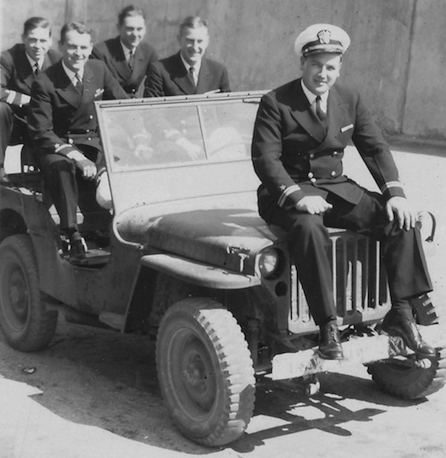
\includegraphics{figures/jeep.png}}\\
(b) \scalebox{.8}{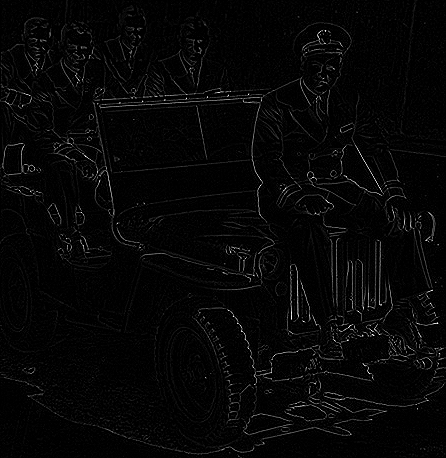
\includegraphics{figures/jeep-edges.png}}
\end{center}
\caption{Edges of an old photograph from World War II.  (a) original, (b) edges as computed by {\tt edges.py}.}
\label{jeepedges}
\end{marginfigure}

The mechanism we're going to use is derived from some serious calculus kung fu called the {\em Laplacian}, but which, in the end, reduces to 4 additions and a subtraction!  The intuition behind the Laplacian is that abrupt changes in brightness indicate edges, such as the transition from the darkness of a uniform to the brightness of a windshield edge.  As we did for blurring and denoising, we are going to slide a 3x3 region around the image to create new pixels at each {\tt x}, {\tt y}. That  means we can reuse our {\tt filter} function---we just need a {\tt laplace} function to pass to {\tt filter}.

To get started, here is the boilerplate code copied from {\tt denoise2.py} but with function name {\tt laplace} (the object of this task) passed as an argument to function {\tt filter}:

\begin{pyverbatim}
from filter import *
# define function laplace here
...
img = open(sys.argv)
img.show()
edges = filter(img, laplace)
edges.show()
\end{pyverbatim}

{\bf Create function} {\tt laplace} that takes region {\tt data} as an argument as usual. Have the function body  return the sum of the North, South, East, and West pixels minus 4 times the middle pixel from our usual region:

\begin{center}
\scalebox{.15}{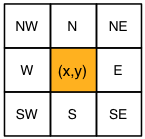
\includegraphics{figures/3x3-region.png}}
\end{center}

\noindent That computation effectively compares the strength of the current pixel with those around it.

\begin{callout}{\bcinfo}
For those familiar with calculus, we are using the second partial derivative (i.e., acceleration) in x and y directions. The first derivative would detect edges even for gradual changes but the second derivative detects only really sharp changes. For a pixel fetching function $f$ operating on a 3x3 region around $(x,y)$, ``applying the {\em Laplacian}'' means computing a filtered image pixel at $x,y$ as:

{\footnotesize $f(x + 1,y) + f(x - 1,y) + f(x,y + 1) + f(x,y - 1) - 4f(x, y)$}

where $f(x,y)$ is equivalent to our {\tt pixels[x,y]}.
\end{callout}

For example, imagine a region centered over a vertical white line. The region might look like:

\begin{center}
\scalebox{.15}{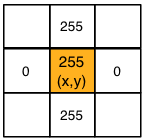
\includegraphics{figures/vertical-line-region.png}}
\end{center}

\marginnote{Be aware of something that Pillow is doing for us automatically when we store values into an image with {\tt pixels[x,y] = v}.  {\bf If {\tt v} is out of range 0..255, Pillow clips {\tt v}}. So, for example, {\tt pixels[x,y] = -510} behaves like {\tt pixels[x,y] = 0} and {\tt pixels[x,y] = 510} behaves like {\tt pixels[x,y] = 255}. It doesn't affect edge detection or any of our other operations in future tasks but I wanted to point out that in a more advanced class we would {\bf scale} these pixel values instead of clipping them. Clipping has the effect of reducing contrast.
}

\noindent The {\tt laplace} function would return $255+255+0+0 - 4 \times 255 = -510$. 

Compare that to the opposite extreme where values are almost the same:

\begin{center}
\scalebox{.15}{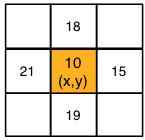
\includegraphics{figures/flat-region.png}}
\end{center}

\noindent The {\tt laplace} function would return $18+19+15+21 - 4 \times 10 = 33$.

Once you have implemented your {\tt laplace} function, give it a try with some of the sample images you have such as the jeep or Obama:

\begin{lstlisting}[style=BashInputStyle]
$ python edges.py obama.png
\end{lstlisting}

It actually does a really good job capturing Obama's outline:\\
~\\

\begin{minipage}{\linewidth}
\makebox[\linewidth]{%
\scalebox{.3}{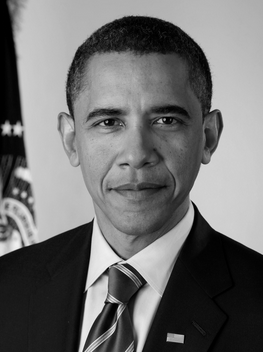
\includegraphics{figures/obama.png}} \scalebox{.3}{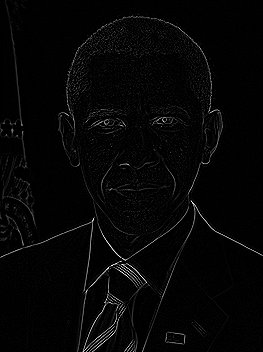
\includegraphics{figures/obama-edges}}
}
\end{minipage}

\begin{callout}{\bcplume}
{\bf Deliverables}. Make sure that {\tt images-}{\em userid}{\tt /edges.py} is correctly committed to your repository and pushed to github. 
\end{callout}

\section{Task 6. Sharpening}

Sharpening an image is a matter of highlighting the edges, which we know how to compute from the previous task. Script {\tt edges.py} computes just the edges so, to highlight the original image, we {\em subtract} that white-on-black edges image from the original.  You might imagine that {\em adding} the edges back in would be more appropriate and it sort of works, but the edges are slightly off. We get a better image by subtracting the high-valued light pixels because that darkens the edges in the original image, such as between the uniform and the windshield. Let's start with the easy stuff:

\begin{marginfigure}
\begin{center}
(a) \scalebox{.6}{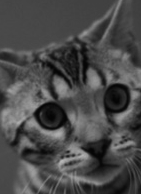
\includegraphics{figures/bonkers-bw-zoom.png}}\\
(b) \scalebox{.6}{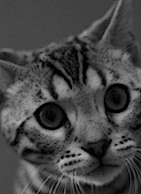
\includegraphics{figures/bonkers-sharp-zoom.png}}
\end{center}
\caption{Bonkers the cat portrait. (a) original and (b) sharpened as computed by {\tt sharpen.py}.}
\label{jeepedges}
\end{marginfigure}

\begin{enumerate}
\item Copy your previous {\tt edges.py} file to new script {\tt sharpen.py}.
\item After {\tt edges = filter(img, laplace)}, add a line that calls a function we'll create shortly called {\tt minus}. {\tt minus} takes two image parameters, {\tt A} and {\tt B} and returns {\tt A-B}.  In our case, pass in the original image and the image you get back from calling {\tt filter(img, laplace)}.
\item Show the result of the {\tt minus} function.
\end{enumerate}

That only leaves the task of {\bf creating function} {\tt minus} to subtract the pixels of one image from the pixels of another image like a 2-D matrix subtraction.  As we did before, we will return a modified version of a copy of an incoming image parameter. (In my solution, I arbitrarily chose to create and return a copy of {\tt A}.) Because you are getting really good at creating functions to manipulate images, the instructions for creating {\tt minus} in this  task are less specific than in previous tasks.  You need to fill in the body of this function:
 
\begin{pyverbatim}
# Return a new image whose pixels are A[x,y] - B[x,y]
def minus(A, B):
	...
\end{pyverbatim}

The mechanism is the same as before: iterating loop variables {\tt x} and {\tt y} across the entire image and processing the pixel at each location. The only difference between this function and {\tt filter} is that we want to operate on individual pixels not 3x3 regions.  In the inner loop, set {\tt pixels[x,y]} to the value of pixel {\tt A[x,y]} minus pixel {\tt B[x,y]}. Don't forget to return the image you filled in.

Here's how to run {\tt sharpen.py} on Bonkers the cat:

\begin{lstlisting}[style=BashInputStyle]
$ python sharpen.py bonkers-bw.png
\end{lstlisting}

\noindent \figref{bonkers3}, \figref{phobos3}, and \figref{jeep3} show some sample transformation sequences with original, {\em Laplacian}, and sharpened images.

\begin{callout}{\bcplume}
{\bf Deliverables}. Make sure that {\tt images-}{\em userid}{\tt /sharpen.py} is correctly committed to your repository and pushed to github. 
\end{callout}

\begin{minipage}{0.8 \linewidth}
\makebox[\linewidth]{%
\scalebox{.35}{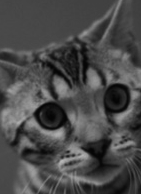
\includegraphics{figures/bonkers-bw-zoom.png}} \scalebox{.35}{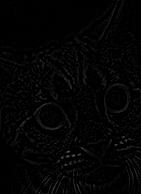
\includegraphics{figures/bonkers-edges-zoom.png}} \scalebox{.35}{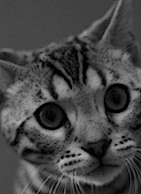
\includegraphics{figures/bonkers-sharp-zoom.png}}
}
\captionof{figure}{Sharpening of a Bonkers the cat. Clockwise: (a) original, (b) edges as computed by {\tt edges.py}, (c) the sharpened image as computed by {\tt sharpen.py}.}
\label{bonkers3}
\end{minipage}

\begin{minipage}{0.8 \linewidth}
\makebox[\linewidth]{%
\scalebox{.45}{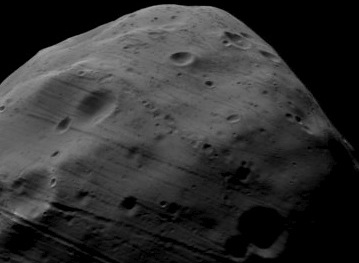
\includegraphics{figures/phobos1.png}}
\scalebox{.45}{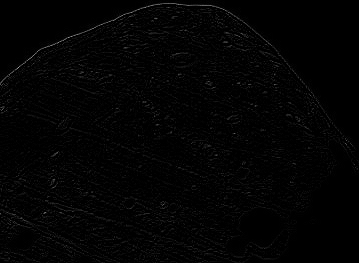
\includegraphics{figures/phobos1-edges.png}}\\
\scalebox{.45}{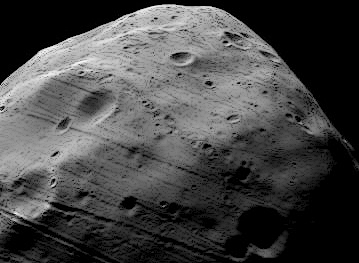
\includegraphics{figures/phobos1-sharp.png}}
}
\captionof{figure}{Sharpening of Phobos asteroid from NASA. Clockwise: (a) original, (b) edges as computed by {\tt edges.py}, (c) the sharpened image as computed by {\tt sharpen.py}.}
\label{phobos3}
\end{minipage}

\begin{minipage}{0.8 \linewidth}
\makebox[\linewidth]{%
\scalebox{.45}{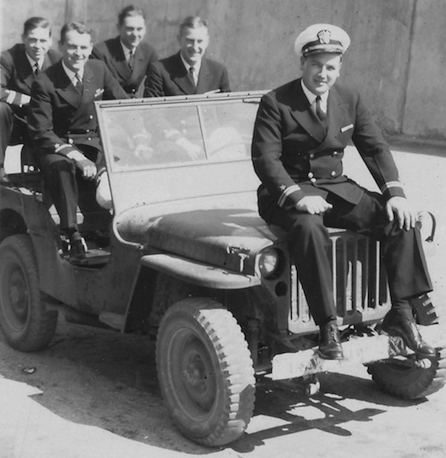
\includegraphics{figures/jeep.png}}
\scalebox{.45}{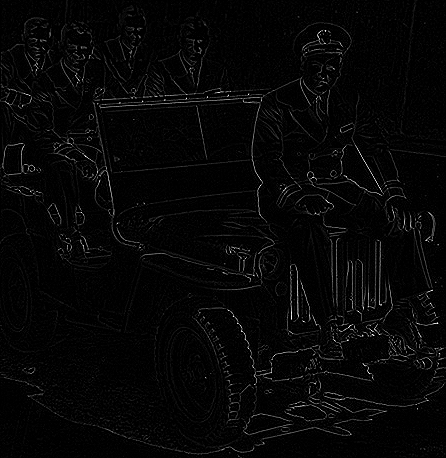
\includegraphics{figures/jeep-edges.png}}\\
\scalebox{.45}{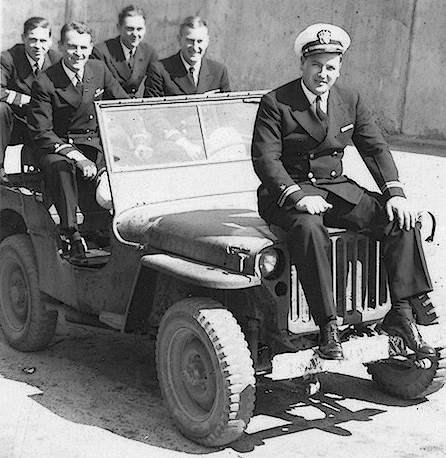
\includegraphics{figures/jeep-sharp.png}}
}
\captionof{figure}{Sharpening of an old photograph from World War II. Clockwise: (a) original, (b) edges as computed by {\tt edges.py}, (c) the sharpened image as computed by {\tt sharpen.py}.}
\label{jeep3}
\end{minipage}

\end{document}
